\documentclass[11pt]{article}

\usepackage[a4paper,margin=1in]{geometry}
\usepackage[T1]{fontenc}
\usepackage[utf8]{inputenc}
\usepackage{lmodern}
\usepackage{amsmath,amssymb,mathtools}
\usepackage{slashed}
\usepackage{booktabs}
\usepackage{array}
\usepackage{graphicx}
\usepackage{xcolor}
\usepackage{hyperref}

\hypersetup{
  colorlinks=true,
  linkcolor=blue!60!black,
  citecolor=blue!60!black,
  urlcolor=blue!60!black
}

\newcommand{\ii}{\mathrm{i}}
\newcommand{\Ds}{D_s}
\newcommand{\Dsone}{D_{s1}}
\newcommand{\Bs}{B_s}
\newcommand{\Bsone}{B_{s1}}
\newcommand{\GeV}{\mathrm{GeV}}
\newcommand{\MeV}{\mathrm{MeV}}
\newcommand{\keV}{\mathrm{keV}}
\newcommand{\qqbar}{\langle\bar q q\rangle}
\newcommand{\ssbar}{\langle\bar s s\rangle}
\newcolumntype{L}[1]{>{\raggedright\arraybackslash}p{#1}}

\title{Radiative Transitions of Strange Heavy Axial Mesons from Light-Cone QCD Sum Rules}
\author{S. Bilmis et al.}
\date{\today}

\begin{document}
\maketitle

\begin{abstract}
We present a light-cone QCD sum-rule analysis of
$\Dsone(2460)\to\Ds\gamma$, $\Dsone(2536)\to\Ds\gamma$, and
$\Bsone(5830)\to\Bs\gamma$.  The calculation keeps explicit strange-quark-mass
terms and includes hard photon emission from both quark lines, two-particle
photon distribution amplitudes, and the three-particle photon-amplitude
corrections induced by the background-gluon term in the quark propagator.  We
separate the basis-current sum rules from the physical-current residue
normalization.  For the charm-strange channel the physical residues are
projected from an $AA/AB/BB$ two-point matrix at the previously determined
mixing angle; for the bottom-strange channel we use Pullin--Zwicky basis-current
inputs followed by a mixed-current diagonalization closure.  Using the modern
lattice normalization of the
leading-twist photon distribution amplitude, we find
$\Gamma[\Dsone(2460)\to\Ds\gamma]=26.71[22.01,32.44]~\keV$,
$\Gamma[\Dsone(2536)\to\Ds\gamma]=1.656[0.457,3.378]~\keV$, and
$\Gamma[\Bsone(5830)\to\Bs\gamma]=1.504[0.818,5.342]~\keV$.
\end{abstract}

\section{Introduction}

Radiative transitions of positive-parity strange heavy mesons probe the
interplay of heavy-quark spin symmetry, light-quark dynamics, and threshold
effects.  The two charm-strange axial states, $\Dsone(2460)$ and
$\Dsone(2536)$, are especially useful because the lower state has a measured
radiative branching fraction \cite{BaBar2006}, while the upper state has a
measured total width but no prominent $\Ds\gamma$ signal \cite{BaBar2011}.  The
bottom-strange state $\Bsone(5830)$ is observed in hadronic spectroscopy
\cite{CMS2018}; its radiative decay has not yet been measured.

The aim of this paper is not only to quote updated numbers, but also to make the
normalization of the calculation unambiguous.  The light-cone OPE gives
transition form factors for basis currents.  The conversion to the physical
$1^+$ states requires the residues of the physical mixed currents.  We therefore
organize the analysis in stages: first compute the axial and tensor basis
amplitudes, then add the photon-DA corrections, and finally apply the
physical-current normalization.

The hierarchy between $\Dsone(2460)\to\Ds\gamma$ and
$\Dsone(2536)\to\Ds\gamma$ was recently emphasized by Bondar and by
Bondar and Milstein \cite{Bondar2025Why,BondarMilstein2025}.  Their
quark-model explanation is that the physical $J=1$ states are mixed spin
configurations and that the E1 amplitudes enter with different relative signs.
Below we show that the same mechanism appears directly in the LCSR
decomposition of the physical amplitudes.

Two photon-input scenarios are considered throughout.  The first is the legacy
magnetic-susceptibility normalization of the photon distribution amplitudes
\cite{Ball:2002ps,Rohrwild2007}.  The second uses the recent lattice
normalization of the leading-twist photon distribution amplitude
\cite{Bacchio2024}.  The latter is our preferred modern scenario; the former is
kept to show continuity with older light-cone sum-rule analyses.

\section{Hadronic Conventions}

We use $p'=p+q$, where $p'$ is the momentum of the initial axial meson, $p$ is the
momentum of the final pseudoscalar meson, and $q$ is the real-photon momentum.
The pseudoscalar interpolating current is
\begin{equation}
  J_5=\bar s\,\ii\gamma_5 Q,\qquad Q=c,b .
\end{equation}
For the axial channel we introduce two basis currents,
\begin{align}
  J^A_\mu &= \bar s\gamma_\mu\gamma_5 Q,\\
  J^B_\mu &= \frac{\ii}{m_Q+m_s}\bar s\sigma_{\mu\alpha}p'^\alpha\gamma_5 Q.
  \label{eq:basis-currents}
\end{align}
The momentum in the tensor current is the initial-state momentum $p'^\alpha$.
The physical-current combinations are
\begin{align}
  J_{1\mu} &= \sin\theta\,J^A_\mu+\cos\theta\,J^B_\mu,\\
  J_{2\mu} &= \cos\theta\,J^A_\mu-\sin\theta\,J^B_\mu ,
  \label{eq:physical-currents}
\end{align}
We use the sector-specific results of our dedicated mixing-angle study
\cite{AlievBilmisSavci2024},
\begin{equation}
\theta_{D_s}=26.6\pm0.6^\circ,\qquad
\theta_{B_s}=38.5\pm0.1^\circ.
\end{equation}
The heavy-quark-limit value $35.3^\circ$ and the interval
$25^\circ\leq\theta\leq45^\circ$ are retained only as benchmark and
sensitivity tests; the latter is not interpreted as a statistical confidence
interval.

The radiative matrix element is parametrized as
\begin{equation}
  \langle P(p)\gamma(q,\varepsilon)|A(p',\eta)\rangle
  =
  eG\left[(\eta\cdot\varepsilon^*)(p\cdot q)
  -(\eta\cdot q)(p\cdot\varepsilon^*)\right].
  \label{eq:e1-definition}
\end{equation}
The corresponding width is
\begin{equation}
  \Gamma(A\to P\gamma)
  =
  \frac{\alpha_{\rm em}}{3}\,G^2
  \left(\frac{m_A^2-m_P^2}{2m_A}\right)^3 .
  \label{eq:width}
\end{equation}

\section{Light-Cone Sum Rule}

The starting correlation function is
\begin{equation}
  \Pi_\mu(p,q)=\ii\int d^4x\,e^{\ii p\cdot x}
  \langle\gamma(q,\varepsilon)|
  T\{\bar s(x)\Gamma_\mu Q(x)\,\bar Q(0)\ii\gamma_5 s(0)\}
  |0\rangle ,
  \label{eq:correlator}
\end{equation}
where $\Gamma_\mu$ is either $J^A_\mu$ or $J^B_\mu$.  We project onto the
gauge-invariant E1 tensor
\begin{equation}
  T_{\mu\nu}=(p\cdot q)g_{\mu\nu}-q_\mu p_\nu .
\end{equation}

The OPE is constructed with quark propagators in an external electromagnetic
field.  Both hard photon emission and soft photon distribution-amplitude terms
are retained.  In addition, the background-gluon insertion in the propagator
generates the three-particle photon-DA terms.  The ordinary vacuum-condensate
pieces of the propagator are not inserted as separate three-point corrections:
in the photon LCSR they enter through photon matrix elements and normalizations
such as $\chi_s\ssbar$.  This is separate from the local two-point sum rules
used to determine decay constants, where ordinary SVZ condensates are part of
the OPE.

After Borel transformation and continuum subtraction the basis-current
amplitudes are denoted $G_A$ and $G_B$.  The charm physical couplings are then
formed as
\begin{align}
  G_{2460} &=
  \frac{\sin\theta\,f_A\,G_A+\cos\theta\,f_B\,G_B}{f_1},\\
  G_{2536} &=
  \frac{\cos\theta\,f_A\,G_A-\sin\theta\,f_B\,G_B}{f_2}.
  \label{eq:stage3}
\end{align}
Here $f_1$ and $f_2$ are obtained by projecting the normalized-current
$AA/AB/BB$ two-point QCD sum-rule matrix at the external $D_s$ angle.  The
LO+$d=3$+$d=5$ Monte Carlo gives
\begin{equation}
f_1=0.4046[0.3799,0.4291]~\GeV,\qquad
f_2=0.1677[0.1594,0.1756]~\GeV.
\end{equation}
Diagonalizing this truncated matrix gives
$30.63[29.94,31.29]^\circ$ only as a diagnostic.  The normalized off-diagonal
residual after the external-angle projection is $0.183[0.142,0.225]$.

Wang's current arXiv v4 result is
$f_A(D_{s1})=0.345\pm0.017~\GeV$ \cite{Wang2015}; the former
$0.245\pm0.017~\GeV$ entry was explicitly corrected.  Reproducing that number
is neither necessary nor sufficient to verify the mixed residues: Wang uses a
pure $J_A$ current and a one-pole ansatz, whereas our $AA$ channel contains the
two physical poles after the mixed-current projection.  We therefore make the
comparison at two levels.  The direct LO+$d=3$+$d=5$ $AA$ OPE evaluated in
Wang's window gives $0.2686[0.2607,0.2768]~\GeV$.  Independently, projecting
our two physical poles back onto $J_A$ gives a Borel-weighted one-pole-equivalent
residue $0.2303[0.2194,0.2418]~\GeV$.  The analytic projection is written in
Appendix~\ref{app:two-point}.  Both numbers are normalization diagnostics;
neither is used as an input or presented as a reproduction of Wang's complete
OPE.

For the bottom-strange channel we use the Pullin--Zwicky basis-current inputs
$f_{\Bsone,A}^{\rm PZ}=0.305\pm0.027~\GeV$ and
$f_{\Bsone}^{T,\rm PZ}=0.285\pm0.027~\GeV$ \cite{PullinZwicky2021}.  These
inputs are converted to physical-current decay constants by the mixed-current
diagonalization closure.  For the observed high-combination state in the
preferred lattice-photon row this gives
$f_1^{(B_s)}=0.430[0.369,0.479]~\GeV$ and
$f_2^{(B_s)}=0.215[0.117,0.292]~\GeV$.  This closure is numerically fragile:
in the nominal central-window lattice ensemble only $245/500$ lower-state and
$236/500$ higher-state trials satisfy the physical covariance condition
$|\rho_{AB}|\leq1$.  The bottom results below are therefore conditional on the
accepted closure samples and await a direct bottom-sector $AA/AB/BB$ two-point
calculation.

\section{Numerical Inputs and Scale Convention}

Table~\ref{tab:inputs-polished} lists the main inputs.  Hadron masses, quark
masses, charges, and $\alpha_{\rm em}$ are taken from PDG summaries
\cite{PDG2024}.  The pseudoscalar decay constants are taken in the lattice
context summarized by FLAG \cite{FLAG2024}.  Photon DAs follow Ball, Braun and
Kivel \cite{Ball:2002ps}; the legacy susceptibility comparison follows
Rohrwild \cite{Rohrwild2007}; the modern photon normalization follows the
lattice result of Bacchio et al. \cite{Bacchio2024}.  The input bookkeeping is
kept in \texttt{inputs\_table.csv} and in the generated citation map
\texttt{outputs/input\_citation\_map.csv}.

The photon-DA normalizations are quoted at $\mu=1~\GeV$, while the quark masses
are the usual $\overline{\rm MS}$ inputs, e.g. $m_s(2~\GeV)$ and $m_c(m_c)$.
This is a standard phenomenological convention rather than a fully matched
single-scale setup.  We therefore treat the lattice photon-normalized scenario
as the preferred modern input and retain the susceptibility scenario as a
comparison with older analyses.

\begin{table}[htbp]
  \centering
  \resizebox{\textwidth}{!}{%
  \begin{tabular}{llll}
    \toprule
    Quantity & Symbol & Value & Source/use\\
    \midrule
    quark masses & $m_c,m_b,m_s$ & $1.27(2),\,4.18(3),\,0.093(11)~\GeV$
      & PDG; explicit $m_s$ terms kept\\
    charm masses & $M_{2460},M_{2536},m_{\Ds}$
      & $2.4595,\,2.53511,\,1.96835~\GeV$ & PDG\\
    bottom masses & $M_{5830},m_{\Bs}$
      & $5.82870,\,5.36692~\GeV$ & PDG/CMS\\
    lower $\Bsone$ diagnostic mass & $M_{\Bsone}^{\rm low}$
      & $5.750(26)~\GeV$ & lattice-inspired diagnostic \cite{Lang2015}\\
    pseudoscalar decay constants & $f_{\Ds},f_{\Bs}$
      & $0.2499,\,0.2303~\GeV$ & FLAG/lattice context\\
    charm mixed residues & $f_1,f_2$
      & $0.4046[0.3799,0.4291],\,0.1677[0.1594,0.1756]~\GeV$
      & fixed-angle $AA/AB/BB$ projection\\
    pure axial benchmark & $f_A(D_{s1})$
      & $0.345(17)~\GeV$ & corrected Wang v4 pure-current check\\
    bottom basis constants & $f_{\Bsone,A}^{\rm PZ},f_{\Bsone}^{T,\rm PZ}$
      & $0.305(27),\,0.285(27)~\GeV$ & Pullin--Zwicky\\
    bottom physical constants & $f_1^{(B_s)},f_2^{(B_s)}$
      & $0.430[0.369,0.479],\,0.215[0.117,0.292]~\GeV$ & this work\\
    legacy photon input & $\chi_s(1~\GeV)$
      & $+3.15(30)~\GeV^{-2}$ & comparison scenario\\
    lattice photon input & $f_{\gamma,s}^{\perp}(1~\GeV)$
      & $-55.1(1.9)~\MeV$ & preferred scenario\\
    \bottomrule
  \end{tabular}%
  }
  \caption{Main numerical inputs used in the analysis.}
  \label{tab:inputs-polished}
\end{table}

\begin{table}[htbp]
  \centering
  \resizebox{\textwidth}{!}{%
  \begin{tabular}{lllll}
    \toprule
    Quantity & Current & Central value & Interval & Interpretation\\
    \midrule
    Wang v4 $f_A$ & pure $J_A$, one pole & $0.345$ & $\pm0.017$ & external benchmark\\
    our direct $AA$ OPE & pure $J_A$ & $0.2686$ & $[0.2607,0.2768]$ & truncation benchmark\\
    projected $AA$ equivalent & $J_A$, two poles & $0.2303$ & $[0.2194,0.2418]$ & one-pole-equivalent diagnostic\\
    $f_1$ & mixed $J_1$ & $0.4046$ & $[0.3799,0.4291]$ & not directly Wang-comparable\\
    $f_2$ & mixed $J_2$ & $0.1677$ & $[0.1594,0.1756]$ & not directly Wang-comparable\\
    $\sin\theta f_1$ & $J_A\to D_{s1}(2460)$ & $0.1812$ & $[0.1692,0.1930]$ & projection diagnostic\\
    $\cos\theta f_2$ & $J_A\to D_{s1}(2536)$ & $0.1498$ & $[0.1424,0.1573]$ & projection diagnostic\\
    \bottomrule
  \end{tabular}%
  }
  \caption{Pure-current and projected-current comparison.  Wang's number,
  our direct truncated $AA$ OPE, and the projected two-pole equivalent do not
  share the same OPE truncation and pole model.  The table is therefore a
  normalization benchmark, not a direct validation of either mixed residue.
  Decay constants are in GeV.}
  \label{tab:residue-benchmark-polished}
\end{table}

\section{Results}

The final predictions are summarized in Table~\ref{tab:results-polished}.  We
quote medians and 16--84 percentile intervals rather than Gaussian means and
standard deviations.  This is important because the $\Dsone(2536)$ and
$\Bsone(5830)$ amplitudes can pass close to zero; their width distributions are
therefore non-Gaussian.

\begin{table}[htbp]
  \centering
  \resizebox{\textwidth}{!}{%
  \begin{tabular}{lllllcc}
    \toprule
    Sector & Decay & Photon input & Mixing & Normalization
      & $G~(\GeV^{-1})$ & $\Gamma~(\keV)$\\
    \midrule
    $D_s$ & $\Dsone(2460)\to\Ds\gamma$ & legacy $\chi_s$
      & $26.6(6)^\circ$ & $f_1=0.405[0.381,0.429]$
      & $-0.500[-0.560,-0.432]$ & $52.39[39.30,66.13]$\\
    $D_s$ & $\Dsone(2536)\to\Ds\gamma$ & legacy $\chi_s$
      & $26.6(6)^\circ$ & $f_2=0.168[0.159,0.175]$
      & $-0.196[-0.250,-0.147]$ & $11.89[6.74,19.34]$\\
    $D_s$ & $\Dsone(2460)\to\Ds\gamma$ & lattice $f_{\gamma,s}^{\perp}$
      & $26.6(6)^\circ$ & $f_1=0.405[0.379,0.430]$
      & $-0.357[-0.393,-0.324]$ & $26.71[22.01,32.44]$\\
    $D_s$ & $\Dsone(2536)\to\Ds\gamma$ & lattice $f_{\gamma,s}^{\perp}$
      & $26.6(6)^\circ$ & $f_2=0.168[0.160,0.175]$
      & $-0.0730[-0.104,-0.0384]$ & $1.656[0.457,3.378]$\\
    $B_s$ & $\Bsone(5830)\to\Bs\gamma$ & legacy $\chi_s$
      & $38.5(1)^\circ$ & $f_2^{(B_s)}=0.206[0.130,0.306]$
      & $-0.116[-0.198,-0.0791]$ & $2.830[1.327,8.273]$\\
    $B_s$ & $\Bsone(5830)\to\Bs\gamma$ & lattice $f_{\gamma,s}^{\perp}$
      & $38.5(1)^\circ$ & $f_2^{(B_s)}=0.215[0.117,0.292]$
      & $-0.0842[-0.159,-0.0621]$ & $1.504[0.818,5.342]$\\
    $B_s$ & $\Bsone^{\rm low}(5750)\to\Bs\gamma$ & legacy $\chi_s$
      & $38.5(1)^\circ$ & $f_1^{(B_s)}=0.427[0.368,0.485]$
      & $+0.278[+0.216,+0.358]$ & $9.178[5.488,16.20]$\\
    $B_s$ & $\Bsone^{\rm low}(5750)\to\Bs\gamma$ & lattice $f_{\gamma,s}^{\perp}$
      & $38.5(1)^\circ$ & $f_1^{(B_s)}=0.433[0.371,0.489]$
      & $+0.385[+0.333,+0.457]$ & $18.16[13.03,27.94]$\\
    \bottomrule
  \end{tabular}%
  }
  \caption{Final form-factor and width predictions.  The lattice photon input
  is the preferred modern normalization; the legacy susceptibility input is
  kept as a comparison with older photon-DA analyses.  The
  $\Bsone^{\rm low}(5750)$ entries are lower-partner diagnostics, not observed
  resonances.  The $B_s$ rows are conditional on the physical samples accepted
  by the basis-input diagonal closure.}
  \label{tab:results-polished}
\end{table}

The preferred lattice-normalized result for $\Dsone(2460)$ is a tens-of-keV
partial width.  In contrast, $\Dsone(2536)$ is highly cancellation sensitive:
the same axial and tensor basis amplitudes enter with the opposite physical
combination in Eq.~\eqref{eq:stage3}, driving the amplitude close to zero for a
wide part of the accepted input range.  The observed $\Bsone(5830)$ behaves
similarly in the bottom sector.  Its median width is at the keV scale after the
physical-current normalization and retains a long upper tail.

Table~\ref{tab:interference-polished} makes this cancellation explicit.  The
entries are the two normalized pieces of Eq.~\eqref{eq:stage3}.  For
$\Dsone(2460)$ both pieces have the same sign and add constructively.  For
$\Dsone(2536)$ they have opposite signs and nearly cancel.  This is the LCSR
version of the Bondar--Milstein explanation of why the $\Dsone(2536)$ radiative
mode is difficult to observe.

\begin{table}[htbp]
  \centering
  \resizebox{\textwidth}{!}{%
  \begin{tabular}{llllccccc}
    \toprule
    Case & Mixing & $A_{2460}$ & $B_{2460}$ & $G_{2460}$
    & $A_{2536}$ & $B_{2536}$ & $G_{2536}$ & $|G_{2460}/G_{2536}|$\\
    \midrule
    previous-study nominal & $26.6^\circ$
      & $-0.0848$ & $-0.2776$ & $-0.3624$
      & $-0.4047$ & $+0.3324$ & $-0.0723$ & $5.01$\\
    truncated-matrix diagnostic & $30.61^\circ$
      & $-0.0963$ & $-0.2668$ & $-0.3631$
      & $-0.3991$ & $+0.3873$ & $-0.0118$ & $30.77$\\
    HQET benchmark & $35.3^\circ$
      & $-0.1093$ & $-0.2533$ & $-0.3626$
      & $-0.3726$ & $+0.4327$ & $+0.0601$ & $6.04$\\
    \bottomrule
  \end{tabular}%
  }
  \caption{Central lattice-photon benchmark at the midpoint of the selected
  transition window.  The $2460$ pieces remain constructive and the $2536$
  pieces remain destructive; the angle changes the distance from the
  cancellation near $31.37^\circ$.  All $G$ values are in $\GeV^{-1}$.}
  \label{tab:interference-polished}
\end{table}

The lower $\Bsone$ row in Table~\ref{tab:results-polished} is retained only as
a model-state diagnostic.  It is not an experimentally established resonance
and is not included in the final experiment--theory comparison.

\begin{figure}[htbp]
  \centering
  
\includegraphics[width=0.82\textwidth]{../outputs/final_window_mc_width_histograms.pdf}
  \caption{Final-window Monte Carlo width distributions with the preferred
  lattice photon normalization and the sector-specific previous-study mixing
  angles.}
  \label{fig:mc-polished}
\end{figure}

\begin{figure}[htbp]
  \centering
  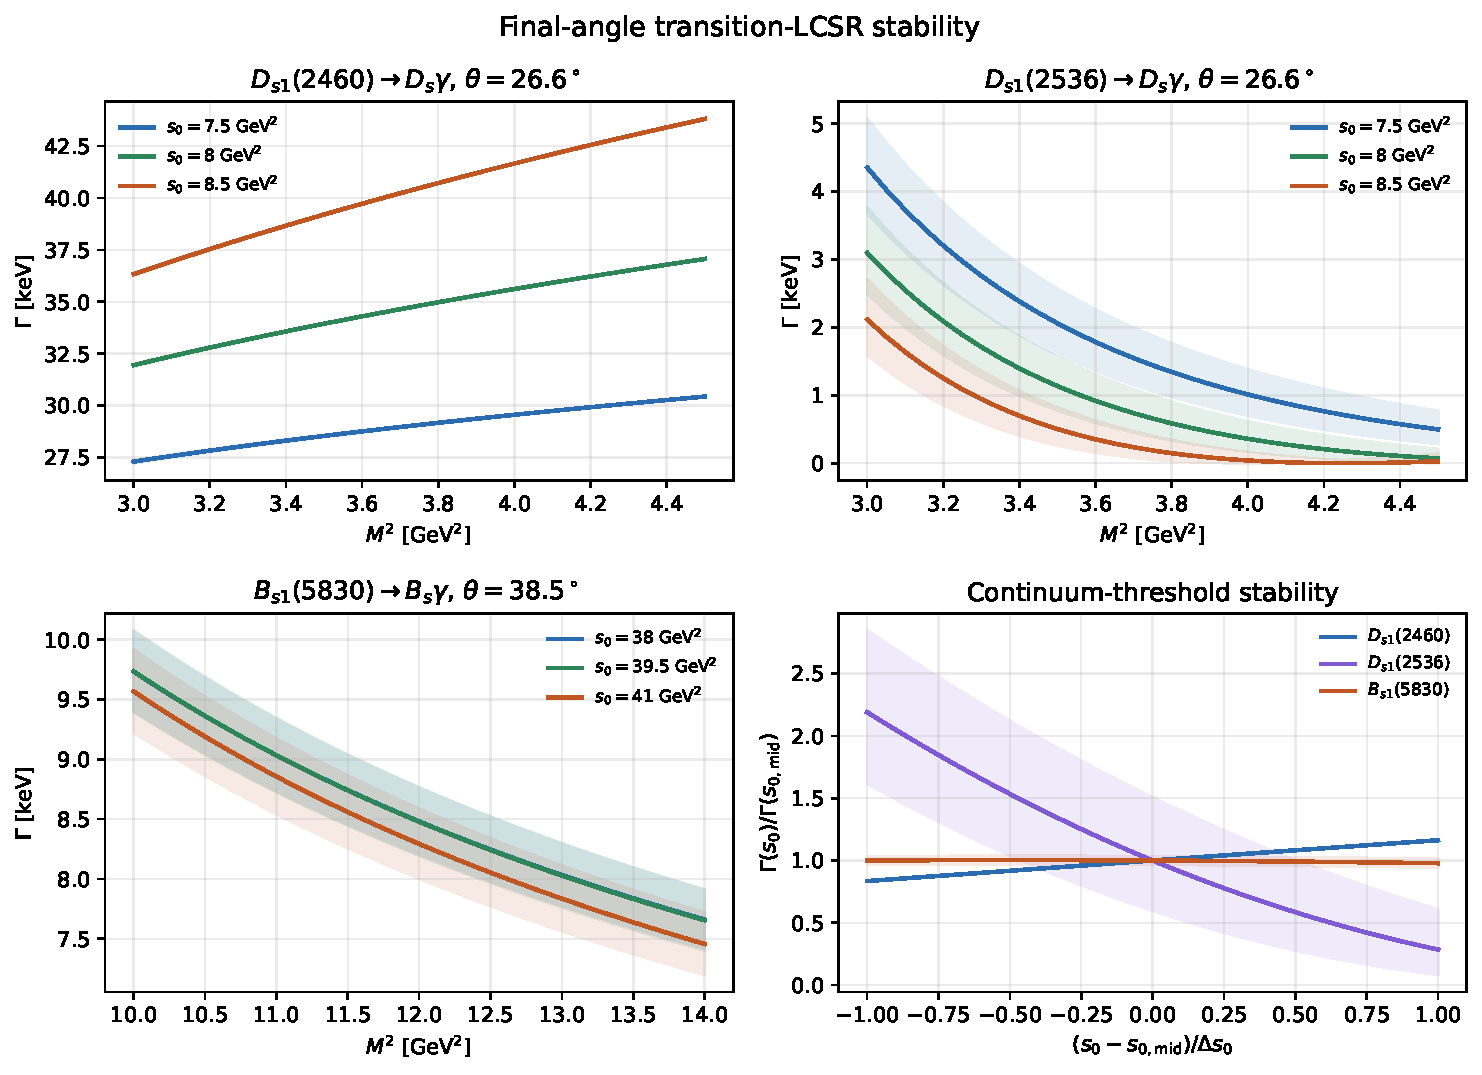
\includegraphics[width=0.96\textwidth]{../outputs/final_angle_stability.pdf}
  \caption{Transition-LCSR stability at the previous-study angles
  $\theta_{D_s}=26.6\pm0.6^\circ$ and
  $\theta_{B_s}=38.5\pm0.1^\circ$.  The curves use the central angles and the
  shaded bands show only their quoted uncertainties.  The physical residues
  are held at their accepted-sample medians to isolate Borel and threshold
  dependence.  The high-state $D_s$ channel is visibly more sensitive because
  its axial and tensor contributions nearly cancel.}
  \label{fig:stability-polished}
\end{figure}

\section{Reproducibility}

Table~\ref{tab:repro-polished} records the source of each headline table and
figure.  The machine-readable version is
\texttt{outputs/manuscript\_reproducibility\_map.csv}.

\begin{table}[htbp]
  \centering
  \resizebox{\textwidth}{!}{%
  \begin{tabular}{llll}
    \toprule
    Manuscript item & Source script & Source output & Purpose\\
    \midrule
    input table & manual bookkeeping & \texttt{inputs\_table.csv} & input values and citations\\
    residue benchmark & \texttt{stage3\_residue\_benchmark\_checks.py} & \texttt{stage3\_residue\_benchmark\_checks.csv} & pure-current validation\\
    main result table & Stage-3 charm and bottom scripts & \texttt{combined\_recommended\_results\_table.csv} & final $G$ and $\Gamma$ values\\
    final comparison table & paper summary scripts & \texttt{bondar\_literature\_comparison\_table.csv}, \texttt{experimental\_comparison\_table.csv} & experiment and literature context\\
    MC width plots & lattice/physical-normalization scan scripts & \texttt{lattice\_fperp\_...pdf}, \texttt{stage3\_bs1\_physical\_...pdf} & uncertainty distributions\\
    final-angle stability & \texttt{final\_angle\_stability\_plots.py} & \texttt{final\_angle\_stability.csv}, \texttt{final\_angle\_stability.pdf} & Borel, threshold, and quoted-angle checks\\
    validation checks & validation and Ward scripts & \texttt{validation\_checks\_summary.txt}, \texttt{ward\_transversality\_check.txt} & limiting cases and gauge structure\\
    interference diagnostic & \texttt{ds1\_interference\_diagnostic.py} & \texttt{ds1\_interference\_diagnostic\_summary.csv} & constructive/destructive amplitude pieces\\
    \bottomrule
  \end{tabular}%
  }
  \caption{Reproducibility map for the headline material in this draft.}
  \label{tab:repro-polished}
\end{table}

\section{Conclusions}

We have computed the radiative transitions of strange heavy axial mesons in a
staged light-cone QCD sum-rule framework.  The calculation includes hard photon
emission from both quark lines, two-particle and three-particle photon
distribution amplitudes, and explicit strange-quark-mass terms.  The charm
residue normalization has been separated from the basis-current OPE and checked
by projection onto the pure axial channel.  This projection is the meaningful
comparison with Wang's one-current calculation; reproducing Wang's one-pole
number is not used as a criterion for the correctness of the two mixed
residues.  The bottom result uses
Pullin--Zwicky basis-current inputs followed by the mixed-current
diagonalization closure; its low physical-sample acceptance makes those
predictions conditional pending a direct bottom-sector two-point matrix.

Table~\ref{tab:conclusion-comparison} gives the requested consolidated
comparison with experiment and representative calculations.  The
$\Dsone(2460)$ result overlaps the original single-current LCSR interval of
Colangelo et al.\ \cite{Colangelo2005}.  Combining our preferred partial width
with the PDG 2025-update branching fraction
$\mathcal B(\Dsone(2460)\to\Ds\gamma)=18\pm4\%$ gives an indicative total width
near $0.15~\MeV$, comfortably below the direct $3.5~\MeV$ upper limit
\cite{PDG2025Update}.  For $\Dsone(2536)$, the measured
$0.92\pm0.05~\MeV$ total width implies
$\mathcal B_\gamma\simeq0.18\%$ at our median, with a 16--84 percentile range
of approximately $0.05$--$0.37\%$.  This is below the indirect
$\mathcal B_\gamma<0.9\%$, or $\Gamma_\gamma<8~\keV$, constraint inferred by
Bondar \cite{Bondar2025Why}.  The observed $\Bsone(5830)$ has no direct
radiative measurement, so that row remains a conditional prediction.

\begin{table}[htbp]
  \centering
  \footnotesize
  \setlength{\tabcolsep}{3pt}
  \begin{tabular}{L{0.24\textwidth}L{0.24\textwidth}
                  L{0.29\textwidth}L{0.16\textwidth}}
    \toprule
    Channel and this work [keV] & Experimental information
      & Selected theory [keV] & Assessment\\
    \midrule
    $\Dsone(2460)\to\Ds\gamma$\newline
      $26.71[22.01,32.44]$
      & $\mathcal B_\gamma=18(4)\%$;\newline
        $\Gamma_{\rm tot}<3.5~\MeV$
        \cite{PDG2025Update}
      & LCSR $19$--$29$ \cite{Colangelo2005};
        QM $3.53$--$17.2$ \cite{GoityRoberts2001,Chen2020Electric}
      & overlaps the earlier LCSR\\
    $\Dsone(2536)\to\Ds\gamma$\newline
      $1.656[0.457,3.378]$
      & $\Gamma_{\rm tot}=0.92(5)~\MeV$ \cite{PDG2025Update};\newline
        indirect $\Gamma_\gamma<8$ \cite{Bondar2025Why}
      & $1.6\pm2.3$ \cite{KornerPirjolSchilcher1993};
        $7$--$61$ (models), $12$ \cite{BondarMilstein2025}
      & compatible with the bound; cancellation sensitive\\
    $\Bsone(5830)\to\Bs\gamma$\newline
      $1.504[0.818,5.342]$
      & no direct radiative measurement \cite{CMS2018}
      & $27$--$56.6$ \cite{LiNiZhong2021,GodfreyMoatsSwanson2016,LuPanWang2016};
        $28$ \cite{BondarMilstein2025}
      & conditional low-width prediction\\
    \bottomrule
  \end{tabular}
  \caption{Consolidated experiment and literature comparison for the preferred
  lattice-photon scenario.  The wide theory spread reflects different
  state assignments, mixing conventions, and normalization schemes.}
  \label{tab:conclusion-comparison}
\end{table}

The scientifically robust conclusion is the interference pattern rather than
an artificially precise high-state number.  The $\Dsone(2460)$ amplitude is
constructive and naturally lies at the tens-of-keV level.  The
$\Dsone(2536)$ amplitude is destructive and the final-angle stability plot
shows enhanced threshold and angle sensitivity near its zero.  The observed
$\Bsone(5830)$ is likewise a cancellation channel, but its absolute
normalization is less secure because a dedicated bottom $AA/AB/BB$ two-point
matrix is not yet available.

\appendix

\section{Explicit analytic light-cone sum rules}
\label{app:lcsr}

\subsection{Correlator, Wick contractions, and propagators}

With $p'=p+q$, the Rohrwild-style external-photon correlator used for either
basis current is
\begin{equation}
 \Pi_\mu^X(p,q)=\ii\int d^4x\,e^{\ii p\cdot x}
 \langle\gamma(q,\varepsilon)|
 T\{J_\mu^X(x)J_5^\dagger(0)\}|0\rangle,\qquad X=A,B .
 \label{eq:app-correlator}
\end{equation}
The hard-emission Wick contraction is
\begin{equation}
 \Pi_{\mu}^{X,\mathrm{hard}}
 =-\ii N_c\!\int\!\frac{d^4k}{(2\pi)^4}
 \operatorname{Tr}\!\left[
 \Gamma_\mu^X S_Q^\gamma(k)\,\ii\gamma_5 S_s^0(k-p)
 +\Gamma_\mu^X S_Q^0(k)\,\ii\gamma_5 S_s^\gamma(k-p)
 \right],
 \label{eq:app-wick}
\end{equation}
where $S_f^0(k)=\ii(\slashed{k}+m_f)/(k^2-m_f^2+\ii0)$.
The light-strange propagator is written without ordinary local-condensate
pieces:
\begin{align}
 \widehat{s^a(x)\bar s^b(0)}={}&
 \delta^{ab}\left[\frac{\ii\slashed{x}}{2\pi^2x^4}
 -\frac{m_s}{4\pi^2x^2}\right]\nonumber\\
 &-\frac{\ii g_s}{16\pi^2x^2}\int_0^1du\,
 \{\bar u\slashed{x}\sigma_{\alpha\beta}
 +u\sigma_{\alpha\beta}\slashed{x}\}
 G_A^{\alpha\beta}(ux)t^A_{ab}\nonumber\\
 &-\frac{\ii e_s\delta^{ab}}{16\pi^2x^2}\int_0^1du\,
 \{\bar u\slashed{x}\sigma_{\alpha\beta}
 +u\sigma_{\alpha\beta}\slashed{x}\}
 F^{\alpha\beta}(ux)\nonumber\\
 &-\frac{m_s}{32\pi^2}\int_0^1du\,
 [g_sG_A^{\alpha\beta}(ux)t^A_{ab}
 +e_s\delta^{ab}F^{\alpha\beta}(ux)]
 \sigma_{\alpha\beta}L_x+\cdots ,
 \label{eq:app-light-propagator}
\end{align}
where $\bar u=1-u$ and
$L_x=\ln(-x^2\mu^2/4)+2\gamma_E$.  The last line is the linear-$m_s$ Wilson
coefficient in one background field; it is not a local condensate.  Setting
$m_s=0$ reproduces the form used by Rohrwild \cite{Rohrwild2007}.

The one-background-field momentum representation used for both heavy and
light lines is
\begin{align}
 S_f^{\mathcal F}(x)=-\ii c_f\int\frac{d^4k}{(2\pi)^4}e^{-\ii k\cdot x}
 \int_0^1du\Bigg[
 &\frac{\slashed{k}+m_f}{2(m_f^2-k^2)^2}
 \mathcal F^{\alpha\beta}(ux)\sigma_{\alpha\beta}\nonumber\\
 &+\frac{ux_\alpha}{m_f^2-k^2}
 \mathcal F^{\alpha\beta}(ux)\gamma_\beta\Bigg],
 \label{eq:app-background-propagator}
\end{align}
with $(c_f,\mathcal F)=(e_f,F)$ for the electromagnetic field and
$(g_s,G)$ for the gluon field.  Equations
\eqref{eq:app-light-propagator}--\eqref{eq:app-background-propagator} show
explicitly that no ordinary local term such as
$-\langle\bar ss\rangle/12$ is inserted into the transition calculation.
The condensate-dependent terms instead occur in nonlocal photon matrix
elements, for example
\begin{align}
 \langle\gamma(q,\varepsilon)|\bar s(x)\sigma_{\mu\nu}s(0)|0\rangle
 ={}&-\ii e e_s\ssbar
 (\varepsilon_\mu q_\nu-\varepsilon_\nu q_\mu)
 \int_0^1du\,e^{\ii\bar u q\cdot x}
 \left[\chi_\gamma\phi_\gamma(u)
 +\frac{x^2}{16}\mathbb A(u)\right]+\cdots .
 \label{eq:app-photon-matrix-element}
\end{align}

\subsection{Double-Borel normalization and axial invariant}

Define
\begin{align}
 \langle0|J_5|P(p)\rangle&=\frac{f_Pm_P^2}{m_Q+m_s},&
 \langle0|J_i^\mu|H_i(p',\eta)\rangle&=f_iM_i\eta^\mu .
\end{align}
After projection onto
$T_{\mu\nu}=(p\!\cdot q)g_{\mu\nu}-q_\mu p_\nu$, the pole contribution is
\begin{equation}
 \widehat T_i^{\rm pole}
 =\frac{f_Pm_P^2}{m_Q+m_s}\,f_iM_iG_i
 \exp\!\left(-\frac{M_i^2}{\mathcal M_1^2}
             -\frac{m_P^2}{\mathcal M_2^2}\right).
 \label{eq:app-pole}
\end{equation}
For $\mathcal M_1^2=\mathcal M_2^2=2M^2$,
\begin{align}
 G_1&=\mathcal N_1(\sin\theta\,\widehat T_A
                   +\cos\theta\,\widehat T_B),\nonumber\\
 G_2&=\mathcal N_2(\cos\theta\,\widehat T_A
                   -\sin\theta\,\widehat T_B),\qquad
 \mathcal N_i=
 \frac{e^{(M_i^2+m_P^2)/(2M^2)}(m_Q+m_s)}
 {M_if_i\,m_P^2f_P}.
 \label{eq:app-physical-lcsr}
\end{align}

Let $E_Q=e^{-m_Q^2/M^2}$, $E_0=e^{-s_0/M^2}$ and $u_0=1/2$.  In the
positive-magnitude susceptibility convention used in the numerical code, the
paper-default axial invariant is
\begin{align}
 \widehat T_A^{\rm RW}={}&
 \int_{(m_Q+m_s)^2}^{s_0}ds\,e^{-s/M^2}\rho_A^P(s)
 +e_s\ssbar(E_Q-E_0)M^2\chi_\gamma\phi_\gamma(u_0)\nonumber\\
 &-e_s\ssbar E_Q\left[
 -\frac14\{\mathbb A(u_0)-8\bar H_\gamma(u_0)\}
 \left(1+\frac{m_Q^2}{M^2}\right)
 -\mathcal I_{\mathcal F_1}(u_0)\right]\nonumber\\
 &+2e_sf_{3\gamma}m_QE_Q\Psi^v(u_0)
 +\mathcal I_A^{\rm em}.
 \label{eq:app-axial-invariant}
\end{align}
Here
\begin{align}
 \bar H_\gamma(u_0)&=\int_0^{u_0}du\int_0^u dv\,h_\gamma(v),&
 \Psi^v(u_0)&=\int_0^{u_0}du\,\psi^v(u),
\end{align}
and
\begin{align}
 \mathcal I_{\mathcal F_1}(u_0)={}&
 \int_0^{1-u_0}\!dv\int_0^{u_0/(1-v)}\!d\alpha_g\,
 \mathcal F_1(u_0-(1-v)\alpha_g,1-u_0-v\alpha_g,\alpha_g)
 \nonumber\\
 &+\int_{1-u_0}^{1}\!dv\int_0^{(1-u_0)/v}\!d\alpha_g\,
 \mathcal F_1(u_0-(1-v)\alpha_g,1-u_0-v\alpha_g,\alpha_g).
 \label{eq:app-f1-integral}
\end{align}
The three-particle combination appearing here is
\begin{equation}
 \mathcal F_1=\mathcal S+\widetilde{\mathcal S}
 -\mathcal T_1-\mathcal T_2+\mathcal T_3+\mathcal T_4
 +2v(-\mathcal S-\mathcal T_3+\mathcal T_2).
\end{equation}
The perturbative density is unambiguously specified by
\begin{align}
 \rho_i(s;m_i,m_j,e_i)={}&-\frac{3e_i}{8\pi^2}
 \Bigg[2m_i\ln\frac{s-m_j^2+m_i^2-\sqrt{\lambda(s,m_j^2,m_i^2)}}
 {s-m_j^2+m_i^2+\sqrt{\lambda(s,m_j^2,m_i^2)}}\nonumber\\
 &+(m_j-m_i)\frac{m_j^2-m_i^2-s}{s^2}
 \sqrt{\lambda(s,m_j^2,m_i^2)}\Bigg],\nonumber\\
 \rho_A^P(s)={}&\rho_s(s;m_s,m_Q,e_s)-\rho_Q(s;m_Q,m_s,e_Q).
 \label{eq:app-rho-a}
\end{align}

\subsection{Tensor invariant and local-scheme separation}

For completeness, the tensor hard density used in the diagonal
double-dispersion prescription can be written
\begin{align}
 \rho_B^P(s)&=e_s\mathcal L(s;m_s,m_Q;a_s,b_s)
              -e_Q\mathcal L(s;m_Q,m_s;a_Q,b_Q),\nonumber\\
 \mathcal L(s;m_i,m_j;a,b)&=-\frac{3}{8\pi^2}\left[
 2a\ln\frac{s-m_j^2+m_i^2-\sqrt{\lambda}}
 {s-m_j^2+m_i^2+\sqrt{\lambda}}
 +\frac{b}{m_i^2}\frac{m_j^2-m_i^2-s}{s^2}\sqrt{\lambda}\right],
 \label{eq:app-rho-b}
\end{align}
where $d=m_Q+m_s$,
\begin{equation}
 a_s=\frac{m_Qm_s}{d},\quad b_s=\frac{m_s^2s}{d},\qquad
 a_Q=\frac{2m_Q^2-m_Qm_s}{d},\quad b_Q=-\frac{m_Q^2s}{d}.
\end{equation}
At the Borel saddle, the two-particle tensor-DA pieces obey
\begin{align}
 \widehat T_B^{\rm tw2+tw4}
 &=\frac{m_Q}{d}\widehat T_A^{\rm tw2+tw4},\nonumber\\
 \widehat T_B^{\rm tw3}
 &=R_v\,\widehat T_A^{\rm tw3},\qquad
 R_v=\frac{3m_P^2+(2\bar u_0+3)p\cdot q}{3m_Qd}.
 \label{eq:app-tensor-2p}
\end{align}
The matched three-particle term is
\begin{align}
 \widehat T_B^{\rm 3p}
 &=\frac{m_Q}{d}\,e_s\ssbar E_Q\,\mathcal I_B^{\rm 3p},\nonumber\\
 \mathcal I_B^{\rm 3p}
 &=\mathcal I_\sigma+
 \left(1+\frac{p\cdot q}{2m_Q^2}\right)(\mathcal I_S+\mathcal I_{T_2})
 +\mathcal I_{T_3}-\frac{p\cdot q}{2m_Q^2}\mathcal I_{T_4},
 \label{eq:app-tensor-3p}
\end{align}
where each $\mathcal I_X$ is the same two-domain light-cone integral as
Eq.~\eqref{eq:app-f1-integral} with the indicated photon DA kernel.
Finally, with
$p^2=m_P^2$ and $p\cdot q=(m_A^2-m_P^2)/2$, the nonlocal electromagnetic
terms are
\begin{align}
 \mathcal I_A^{\rm em}
 &=e_Q\ssbar(E_Q-E_0)
 \frac{2(m_P^2-m_A^2)}{M^2}P_\gamma,\nonumber\\
 \mathcal I_B^{\rm em}
 &=e_Q\ssbar(E_Q-E_0)\left[
 (r_0-r_S)\frac{25}{16}-r_T\frac{5}{16}
 +2r_0\frac{m_P^2-m_A^2}{M^2}P_\gamma\right],
 \label{eq:app-em-terms}\\
 P_\gamma&=\ln8-\frac{1181}{320},\qquad
 r_0=\frac{m_Q}{d},\quad
 r_S=\frac{m_Q^2+\tfrac12p\cdot q}{m_Qd},\quad
 r_T=\frac{-m_Q^2+m_P^2+\tfrac32p\cdot q}{m_Qd}.\nonumber
\end{align}
Equations \eqref{eq:app-rho-b}--\eqref{eq:app-em-terms}, together with
\begin{equation}
 \widehat T_B^{\rm RW}=\int ds\,e^{-s/M^2}\rho_B^P
 +\widehat T_B^{\rm tw2+tw4}
 +\widehat T_B^{\rm tw3}
 +\widehat T_B^{\rm 3p}
 +\mathcal I_B^{\rm em},
\end{equation}
are the explicit tensor prescription used in the Python analysis.

\begin{table}[htbp]
 \centering
 \resizebox{\textwidth}{!}{%
 \begin{tabular}{lll}
  \toprule
  Contribution & Rohrwild default & Colangelo comparison\\
  \midrule
  ordinary local transition condensate & absent & retained for $J_A$\\
  $\mathcal S_\gamma,\mathcal T_4^\gamma$ & included nonlocally & not added separately\\
  gluonic photon DAs & included & included through $\mathcal F_1$\\
  local condensates in two-point $f_i$ sum rules & required & required\\
  local plus electromagnetic term together & forbidden double counting & forbidden double counting\\
  \bottomrule
 \end{tabular}
 }
 \caption{Separation of the transition and two-point condensate prescriptions.}
 \label{tab:app-local-schemes}
\end{table}

The alternative Colangelo axial invariant is obtained by removing
$\mathcal I_A^{\rm em}$ from Eq.~\eqref{eq:app-axial-invariant} and adding
\begin{equation}
 e_QE_Q\ssbar\left[1-\frac{m_Qm_s}{M^2}
 +\frac{m_s^2}{2M^2}\left(1+\frac{m_Q^2}{M^2}\right)\right].
 \label{eq:app-colangelo-local}
\end{equation}
The two terms are alternatives and are never summed.  In our rotation
convention the exact pure-axial Colangelo limit is
\begin{equation}
 \theta=\frac{\pi}{2},\qquad J_1=J_A,\qquad
 G_1=\frac{e^{(M_1^2+m_P^2)/(2M^2)}(m_Q+m_s)}
 {M_1f_A\,m_P^2f_P}\widehat T_A .
 \label{eq:app-colangelo-limit}
\end{equation}
Thus the agreement in analytic structure is exact at the pure-current point;
with the Colangelo inputs our numerical pure-$A$ width interval is
$20.51$--$33.26~\keV$, overlapping their $19$--$29~\keV$ result.

\section{Explicit \texorpdfstring{$AA/AB/BB$}{AA/AB/BB} two-point sum rules}
\label{app:two-point}

For $i,j\in\{A,B\}$,
\begin{equation}
 \Pi_{ij}^{\mu\nu}(p')=\ii\int d^4x\,e^{\ii p'\cdot x}
 \langle0|T\{J_i^\mu(x)J_j^{\nu\dagger}(0)\}|0\rangle
 =\left(-g^{\mu\nu}+\frac{p'^\mu p'^\nu}{p'^2}\right)
 \Pi_{ij}(p'^2)+\cdots .
\end{equation}
Let $d=m_Q+m_s$ and
$\lambda(s)=[s-(m_Q+m_s)^2][s-(m_Q-m_s)^2]$.  The exact-mass LO spectral
matrix is
\begin{align}
 \rho_{AA}(s)&=\frac{\sqrt\lambda}{8\pi^2}\left[
 2-\frac{m_Q^2+m_s^2+6m_Qm_s}{s}
 -\frac{(m_Q^2-m_s^2)^2}{s^2}\right],\nonumber\\
 \rho_{AB}(s)&=\rho_{BA}(s)=\frac{\sqrt\lambda}{8\pi^2}
 \frac{3(m_s-m_Q)(d^2-s)}{ds},\nonumber\\
 \rho_{BB}(s)&=\frac{\sqrt\lambda}{8\pi^2}
 \frac{-(d^2-s)(2m_s^2-4m_Qm_s+2m_Q^2+s)}{d^2s}.
 \label{eq:app-two-point-rho}
\end{align}
With $C_3=\ssbar$ and
$C_5=\langle\bar s g_s\sigma\!\cdot\!G s\rangle$, the common
LO+$d=3$+$d=5$ Borel matrix is
\begin{equation}
 \widehat\Pi(M^2,s_0)=
 \int_{d^2}^{s_0}ds\,e^{-s/M^2}\rho(s)
 +e^{-m_Q^2/M^2}
 [C_3(\mathcal Q_0+\mathcal Q_1+\mathcal Q_2)+C_5\mathcal Q_5],
 \label{eq:app-two-point-matrix}
\end{equation}
where
\begin{align}
 \mathcal Q_0&=
 \begin{pmatrix}m_Q&m_Q^2/d\\m_Q^2/d&m_Q^3/d^2\end{pmatrix},\nonumber\\
 \mathcal Q_1&=
 \begin{pmatrix}
 -\dfrac{m_sm_Q^2}{2M^2}&
 \dfrac{m_sm_Q(1-m_Q^2/M^2)}{2d}\\
 \dfrac{m_sm_Q(1-m_Q^2/M^2)}{2d}&
 \dfrac{m_sm_Q^2(1-m_Q^2/(2M^2))}{d^2}
 \end{pmatrix},\nonumber\\
 \mathcal Q_2&=
 \begin{pmatrix}
 \dfrac{m_s^2m_Q^3}{2M^4}&
 \dfrac{m_s^2(m_Q^4/M^4-m_Q^2/M^2-1)}{2d}\\
 \dfrac{m_s^2(m_Q^4/M^4-m_Q^2/M^2-1)}{2d}&
 \dfrac{m_s^2(m_Q^5/(2M^4)-m_Q^3/M^2)}{d^2}
 \end{pmatrix},\nonumber\\
 \mathcal Q_5&=
 \begin{pmatrix}
 -\dfrac{m_Q^3}{4M^4}&
 -\dfrac{m_Q^4/M^4-m_Q^2/M^2-1}{4d}\\
 -\dfrac{m_Q^4/M^4-m_Q^2/M^2-1}{4d}&
 -\dfrac{m_Q^5/(4M^4)-m_Q^3/(2M^2)}{d^2}
 \end{pmatrix}.
 \label{eq:app-q-matrices}
\end{align}
These local condensates are required because this is an ordinary two-point
SVZ sum rule; their use does not contradict their exclusion from the
external-photon transition LCSR.

Writing $s_\theta=\sin\theta$ and $c_\theta=\cos\theta$, the physical
invariants are
\begin{align}
 \widehat\Pi_{11}&=s_\theta^2\widehat\Pi_{AA}
 +c_\theta^2\widehat\Pi_{BB}
 +2s_\theta c_\theta\widehat\Pi_{AB},\nonumber\\
 \widehat\Pi_{22}&=c_\theta^2\widehat\Pi_{AA}
 +s_\theta^2\widehat\Pi_{BB}
 -2s_\theta c_\theta\widehat\Pi_{AB},\nonumber\\
 \widehat\Pi_{12}&=s_\theta c_\theta
 (\widehat\Pi_{AA}-\widehat\Pi_{BB})
 +(c_\theta^2-s_\theta^2)\widehat\Pi_{AB}.
 \label{eq:app-rotated-pi}
\end{align}
The decay-constant sum rules are therefore
\begin{align}
 f_1^2(\theta)&=\frac{e^{M_1^2/M^2}}{M_1^2}
 [s_\theta^2\widehat\Pi_{AA}
 +c_\theta^2\widehat\Pi_{BB}
 +2s_\theta c_\theta\widehat\Pi_{AB}],\nonumber\\
 f_2^2(\theta)&=\frac{e^{M_2^2/M^2}}{M_2^2}
 [c_\theta^2\widehat\Pi_{AA}
 +s_\theta^2\widehat\Pi_{BB}
 -2s_\theta c_\theta\widehat\Pi_{AB}].
 \label{eq:app-decay-constants}
\end{align}
We insert the previous-study angle $26.6\pm0.6^\circ$
\cite{AlievBilmisSavci2024} here; we do not refit it in the radiative paper.
Setting $\widehat\Pi_{12}=0$ gives the
$30.63[29.94,31.29]^\circ$ truncation diagnostic quoted in the text.

\subsection{Projection onto Wang's pure axial channel}

Inverting the physical rotation gives $J_A=s_\theta J_1+c_\theta J_2$.
Consequently the two-pole hadronic representation of the pure-$AA$ invariant is
\begin{equation}
 \widehat\Pi_{AA}^{(2\,{\rm pole})}
 =s_\theta^2 f_1^2M_1^2e^{-M_1^2/M^2}
 +c_\theta^2 f_2^2M_2^2e^{-M_2^2/M^2}.
 \label{eq:app-aa-two-pole}
\end{equation}
For comparison with a one-pole result normalized at $M_1$, define only as a
diagnostic
\begin{equation}
 f_{A,\mathrm{eq}}^2(M^2)=
 \frac{e^{M_1^2/M^2}}{M_1^2}
 \widehat\Pi_{AA}^{(2\,{\rm pole})}.
 \label{eq:app-wang-projection}
\end{equation}
The accepted two-point samples give
$f_{A,\mathrm{eq}}=0.2303[0.2194,0.2418]~\GeV$, while the separate direct
$AA$ OPE in Wang's window gives
$0.2686[0.2607,0.2768]~\GeV$ and Wang quotes
$0.345\pm0.017~\GeV$ \cite{Wang2015}.  The three quantities test related
normalization scales but are not identical calculations: the first uses two
physical poles, the second uses our stated truncated OPE, and the third uses
Wang's one-pole OPE.  This is why the comparison is useful but cannot by itself
prove or disprove the mixed-current result.

\section*{Acknowledgments}

To be added.

\bibliographystyle{unsrt}
\bibliography{references}

\end{document}
